\documentclass{article}
\usepackage[nonumberlist]{glossaries}
\usepackage{graphicx}

\makeglossaries

\newglossaryentry{Director}
{
    name = {Director},
    description = {The AI responsible for moving the enemy towards and away from
    the player and directing the enemy to different spots on the map.}
}

\newglossaryentry{NavMesh}
{
    name = {Navigation Mesh},
    description = {The area in which the AI of the game is allowed to move.}
}

\newglossaryentry{ESenses}
{
    name = {Enemy senses},
    description = {What the enemy can see or get information from.}
}

\newglossaryentry{StateMachine}
{
    name = {StateMachine},
    description = {The software design pattern used to model the logic of the enemy AI.}
}

\newglossaryentry{State}
{
    name = {State},
    description = {The possible modes that the state machine can exist in. States dictates
    the current enemy behavior.}
}

\newglossaryentry{AI}
{
    name = {Artificial Intelligence},
    description = {A set of rules that dictates how the game element reacts to different game
    elements within the game.}
}

\newglossaryentry{GE}
{
    name = {Game Element},
    description = {An umbrella term to describe something that is a part of the game.}
}

\newglossaryentry{Sound}
{
    name = {Sound Mechanic},
    description = {A game mechanic where the player makes a sound while moving allowing the 
    enemy to move towards the sound in order to hunt the player.}
}

\begin{document}

\section*{General}
For this prototype I want to make an enemy AI that influences the player
by acting as an obstacle to stop the player from completing their tasks.

\section*{Mechanics}
The prototype will be a continuation of the previous prototype
thus the mechanics will be the same as in the previous prototype.
Small overview of the mechanics.
\begin{itemize}
    \item Player can move with WASD.
    \item Player can sprint with LShift.
    \item Player can interact with Space.
    \item Player can toggle light with R.
\end{itemize}
\subsection*{New Mechanics}
The player will be able to crouch with the left control key to help
them hide from the enemy.
A sound mechanic was added during the process of the prototype, because the
enemy can then hear the player in order to hunt the player better.

\section*{Challenges}
\subsection*{Player Challenges}
The player will need to use the game mechanics to avoid the enemy, while
trying to get their objectives complete. This includes distracting the 
enemy, hiding from the enemy, and moving around the enemy. 
Since the focus of this prototype is on the enemy AI the main challenges
that the player needs to face are challenges based around the enemy AI.

\subsection*{Enemy Challenges}
The enemy will act like a player with different objectives from the actual 
player. The enemy objectives will be to stop the player. The only mechanics
that the enemy has is movement, some senses to detect the player and a 
director AI that will help it. If the enemy hits the player the enemy will win.


\section*{Hypothesis}
How will the change of a horror aesthetic to a greybox aesthetic affect how the player 
interacts with the game when the game has a horror game enemy AI and other horror elements? 


\section*{Goals}
Make an enemy AI that reacts to the player and changes
its behavior according to the player's actions, which in turn
will change the way that the player reacts to the enemy AI.
Some of these reactions include
\begin{itemize}
    \item Patrolling an area more if the player frequents that area. 
    \item Learning the players next objective and then trying to stop
    the player from completing that objective.
    \item Possibly moving the players next objective to stop them from
    completing it.
\end{itemize}






\section*{Enemy AI}
The enemy AI will run with a finite state machine, due to the low complexity
of the prototype the finite state machine will work because the number of 
transitions is low between the 3 states.
(What will the speed be of the enemy in each state.)
The Enemy AI will have 3 total senses. One sense to see the player when there
is light, one sense to see the player when there is no light, one sense
to hear the player.
\subsection*{Enemy States}
\subsubsection*{Idle}
The enemy will randomly move around the map.
In this state the enemy will listen for sounds from the player. If any
sound is heard the enemy will go to the position they heard the sound 
and continue idling.
If the enemy is too far from the player the director will send the enemy
closer to the player.
If the enemy is too close to the player for too long then the director
will send the enemy further from the player.
If the enemy sees the player they will enter the chase state.

\subsubsection*{Chase}
The enemy will constantly walk towards the last seen player's position. If the enemy
loses sight of the player they will listen for player sounds and then the
enemy will go to the position of the sound.
If no sound is heard and the enemy can't see the player the enemy will then
enter the guard state. 
If the enemy sees the player enter a hiding spot the enemy will force the player out of the hiding spot.

\subsubsection*{Guard}
If there is an objective that the player must complete nearby the enemy will
move to that objective and then constantly look in an area around that objective.
If there is no objective nearby the enemy will enter the idle state.
If the enemy hears a sound it will move towards that sound and will guard the
area where the sound was heard. The enemy will then move back to the objective
and continue to guard it until the guard time runs out. The enemy will then return
to the idle state when the guard time runs out.

\section*{Director AI}
The director will be responsible for keeping track of how annoying the enemy
is currently being towards the player, thus the director will know where the
player and enemy is at all times.
This will be done by keeping track of an annoyance meter. 
Certain actions that the enemy does will increase or decrease the annoyance meter.
If the enemy is near the player the annoyance meter will increase while if the enemy
is far from the player the annoyance meter will decrease.
Certain actions the enemy does will increase the annoyance meter. If the enemy is
in the guard state the annoyance meter will go up.
The annoyance meter will not change when the enemy is in the chase state.
If the annoyance meter is full the director will make the enemy walk away from the
player.
If the annoyance meter is empty the director will make the enemy walk towards the
player.
The director will give the enemy nearby player objectives when needed.


\section*{Genre}
The genre of the prototype is survival horror. This is because the player will have to
survive against an enemy AI while trying to accomplish some sort of arbitrary goal.

\section*{Games with dynamic AI systems}
\subsection*{Alien: Isolation}
There are two parts to the AI in Alien: Isolation that is the Director AI and the
Alien AI. The Director AI knows where the alien and player are at all time, but 
it never communicates this to the Alien AI. 
Alien: Isolation is a horror game thus the player needs to be scared, but if the player
is scared the entire time they would just give up. This lead to the Director keeping track
of a menace meter. The menace meter tells the Director when it should get the Alien to 
back off from the player and allow the player some breathing room and time to progress.
The Alien AI can only act on what it senses, this leads the AI feel like its hunting the
player. This is due to the Alien not moving around optimally and taking its time to move
to its destination. 
The Alien can also respond to the player's action if the player makes too much noise and if
the Alien is close enough to sense that noise.
The Alien has different sensors, visual, auditory and touch. The Alien acts on these senses
to try and kill the player.
The Alien AI is made form a behavior tree.



The parts of Alien: Isolation that I will use in my game will be the similar to the Director AI
and the Alien AI. I will have the Director AI keep track of an annoyance meter and direct an Enemy
AI to and away from the player. The Enemy will have a sound sensor and a vision range which it will
use to defeat the player. Unlike the Alien AI which uses a behavior tree the Enemy AI in the prototype
will use a finite state machine. This is because recreating a behavior tree needs a lot of conditions
just to get to the behavior that the AI needs to do at the moment and if made incorrectly can worsen
performance. The finite state machine can get complex if there are too many states, but this will
not happen due to only 3 states being planned for the prototype.



\section*{Micro Design}
The enemy AI will cause moment to moment gameplay by influencing the
player's decision making through the different enemy states. This will cause
the player to either avoid certain areas or delay doing certain tasks
because the enemy is currently obstructing those game elements.
The enemy direct will help with the moment to moment gameplay by
giving the player some breathing time when the enemy is bothering the player
too much or when the enemy is barely bothering the player at all.
The player mechanics will be refined to give more feedback to the
player that they are currently using a mechanic. This includes moving the camera
a bit outward when running and moving the camera a bit inward when crouching.


\section*{Process}
StateMachine for the enemy is being made while following the layout of the youtube videos.
Senses for enemy is being made. 3 Senses have been decided on. Light sense which is what the
enemy can see when it is light. Dark sense which is what the enemy can see when there is no light.
Always sense which is what the enemy can always see.
\newline
During the development of the enemy, when the player is hiding in a hiding spot and the enemy is nearby
the Director will try to send the enemy away, but because the random spot the director chooses to send
the enemy away to can be outside of the NavMesh causing the enemy to move near the player. This gives the
idea that the enemy is searching the area for the player. The director can also send the enemy around
to the back of the player, but this is random. This does give the feeling of the enemy trying to get the 
jump on the player.
\newline
Adding Devtools to more easily see how the enemy moves and what the enemy is currently doing. This also will
help to show off the enemy AI.
\newline
Sound manager is being made while following a youtube video [8]. Some changes from the video will be made. Audio
will only be added to the player and enemy footsteps, because this communicates to the player when they make
a sound the enemy can hear and it communicates to the player how far away the enemy currently is from them.
\newline
Changed the map from a smaller map with only one goal to a bigger map with 3 goals to better show off the 
enemy guard state. 
\newline
Added lights to the new map to allow the player to see more of the map while also giving them a light source 
other than the player light.
\newline
The camera shakes while crouching or sprinting, this is not intended but it adds a sense of anxiety to the
character which fits with the horror theme.
\newline
A small tutorial area was added to the map in order to help the player with the SoundMechanics added.
\newline
Devtools have been added to help show off the enemy AI. 


\begin{figure}[ht!]
    \centering
    \begin{minipage}[b]{0.4\textwidth}
        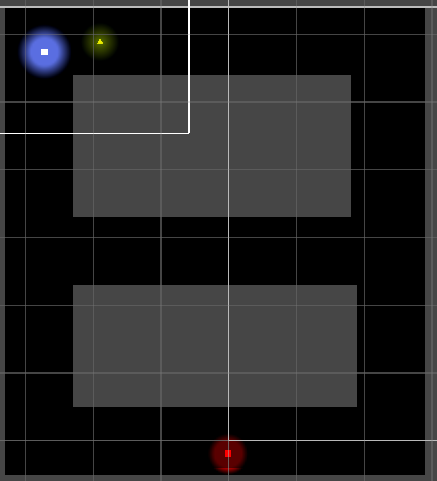
\includegraphics[width=\textwidth]{Images/InitialMap.png}
        \caption{Initial Map}
        \label{img:InitialMap}
    \end{minipage}
    \hfill
    \begin{minipage}[b]{0.4\textwidth}
            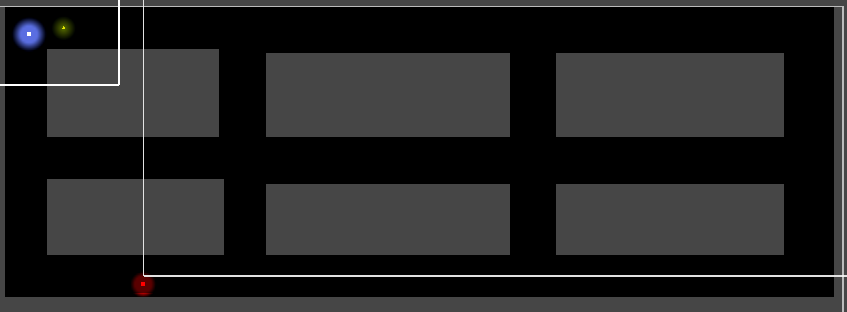
\includegraphics[width=\textwidth]{Images/ExpandedMap.png}
            \caption{Expanded Map}
            \label{img:ExpandedMap}
    \end{minipage}
\end{figure}

\begin{figure}[ht!]
    \centering
    \begin{minipage}[b]{0.4\textwidth}
        
\includegraphics[width=\textwidth]{Images/FinishedMap.png}
        \caption{Finished Map}
        \label{img:FinishedMap}
    \end{minipage}
    \hfill
    \begin{minipage}[b]{0.4\textwidth}
            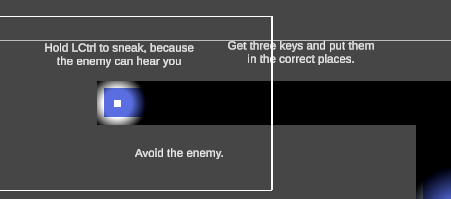
\includegraphics[width=\textwidth]{Images/TutorialArea.png}
            \caption{Tutorial Area}
            \label{img:TutorialArea}
    \end{minipage}
\end{figure}

\newpage
\subsection*{Hypothesis in prototype}
The horror elements added that where talked about in the hypothesis were:
\begin{itemize}
    \item Limited vision.
    \item Enemy AI that tries to hunt the player.
    \item Limited actions to take against enemy.
    \item Ominous footsteps from enemy.
    \item Urgency to run when the enemy can see you.
\end{itemize}

\subsection*{Mechanic balance}
The sprint time on the player was tweaked as more of a sprint burst so that the player can outrun the enemy,
but only if they are in the correct position of the map to do so. 
This is a positive feedback loop which encourages the player to avoid the enemy instead of trying to confront it.
If the enemy sees the player enter a hiding spot the enemy will take the player out of the hiding spot and end the game
this forces the player to stop being chased by the enemy before they can hide.
The player can hide from the enemy by turning off their light and crouching but they still should not get too close, 
because the enemy still has a sense to stop the player form just constantly hiding form the enemy.

\section*{Reflection}
During the prototype the StateMachine helped a lot with the enemy logic and AI. If the enemy AI will get more complicated in 
the future then a different design pattern needs to be used or I need to keep track of all of the transitions between the enemy
states to allow for more complex behavior form the enemy.
The most annoying part of the enemy AI was how similar the Guard and Idle state are where they both get a random movement spot,
but the Guard state gets a random point around a goal while the Idle state gets a random point around the enemy. This caused
the code of both of the states to be almost identical , but it has small differences which can get out of hand when not properly
kept track of.
These elements that I need to keep track of have helped me with documentation of the code, which in turn makes it easier to code.
I will need to keep updating this document the more the the project grows.

\subsubsection*{Goal}
The goal of the prototype was achieved, because I made an enemy AI that uses a StateMachine and successfully changes from one state to
another to hinder the player by patrolling areas, chasing the player and guarding specific areas. This will cause the player to change their
moment to moment gameplay in order to avoid the enemy.

\newpage
\subsubsection*{Hypothesis}
While the game still has the horror element the block aesthetic does hold back the horror of the game. This may just be personal preference, but
if the aesthetic of the game follows a more horror aesthetic the game may be able to be better at scaring the player.

\section*{References}
[1]T. Thompson, “Revisiting the AI of Alien: Isolation,” Aiandgames.com, May 20, 2020. https://www.aiandgames.com/p/revisiting-alien-isolation
\newline
[2]T. Thompson, “The Perfect Organism: The AI of Alien: Isolation,” Game Developer, Oct. 31, 2017. https://www.gamedeveloper.com/design/the-perfect-organism-the-ai-of-alien-isolation
\newline
[3]C. Simpson, “Behavior Trees for AI: How They Work,” Game Developer, Jul. 18, 2014. https://www.gamedeveloper.com/programming/behavior-trees-for-ai-how-they-work
\newline
‌[4]“Tech Breakdown: AI with Finite State Machines,” Littlepolygon.com, Nov. 18, 2024. https://blog.littlepolygon.com/posts/fsm/
\newline
‌[5]Sasquatch B Studios, “A Better Way to Code Your Characters in Unity | Finite State Machine | Tutorial,” YouTube, May 18, 2023. https://www.youtube.com/watch?v=RQd44qSaqww
\newline
‌[6]Sasquatch B Studios, “Enhance Your Game: EASY Enemy Logic Using Scriptable Objects (State Machine PART 2) | Unity Tutorial,” YouTube, May 25, 2023. https://www.youtube.com/watch?v=iOYo7flBUW4
\newline
‌[7]“How to Add a Field of View for Your Enemies [Unity Tutorial],” www.youtube.com. https://www.youtube.com/watch?v=j1-OyLo77ss
\newline
‌[8]Sasquatch B Studios, “How To Add Sound Effects the RIGHT Way | Unity Tutorial,” YouTube, Dec. 08, 2022. https://www.youtube.com/watch?v=DU7cgVsU2rM
\newline
‌[9]“Pixabay,” Pixabay.com, 2024. https://pixabay.com/sound-effects/search/footsteps/
‌
\newpage
\glsaddall
\printglossary

\end{document}